\subsection{Poda alfa-beta}
\label{ssec:poda_alfa_beta}
Esta sección estudia la técnica de la poda alfa-beta como una mejora del algoritmo minimax.
También define los agentes que emplearán esta estrategia, que al igual que ocurría con minimax serán dos: uno con límite de profundidad en la búsqueda y otro con un límite en el tiempo de cómputo.

\bigskip
La \textbf{poda alfa-beta} calcula el mismo movimiento que devolvería minimax sin necesidad de examinar todos los nodos en el árbol de juegos, es decir, poda las ramas del árbol que no influyen en la decisión final.

Esta estrategia dispone de dos parámetros ($\alpha$ y $\beta$) que describen los límites sobre los valores que se propagan hacia arriba en el árbol:
\begin{itemize}
	\item $\alpha$ es el valor de la mejor opción (es decir, el valor más alto) que se ha encontrado hasta ahora en cualquiera de los estados elegidos para \textit{MAX}. 
	\item $\beta$ es el valor de la mejor opción (es decir, el valor más bajo) que se ha encontrado hasta ahora en cualquiera de los estados elegidos para \textit{MIN}.
\end{itemize}
La poda alfa-beta realiza una búsqueda primero en profundidad, con retroceso y de izquierda a derecha.
Para cada nodo se considera un intervalo de posibles valores [$\alpha$, $\beta$].
La búsqueda actualiza estos valores según recorre el árbol: actualiza el valor $\alpha$ (en los nodos \textit{MAX}) y el valor $\beta$ (en los nodos \textit{MIN}).
Cuando encuentra un nodo con un valor peor que su antecesor, la búsqueda se detiene y esa rama del árbol no se examina.
Así, se puede podar:
\begin{itemize}
\renewcommand{\labelitemi}{-}
	\item Debajo de un nodo \textit{MIN} cuando un nodo \textit{MAX} antecesor suyo tenga un valor $\alpha \geq \beta$; lo que se conoce como \textbf{corte $\alpha$}.
	\item Debajo de un nodo \textit{MAX} cuando un nodo \textit{MIN} antecesor suyo tenga un valor $\beta \leq \alpha$; lo que se conoce como \textbf{corte $\beta$}.
\end{itemize}

La figura~\ref{fig:alfabeta} muestra el funcionamiento de la poda alfa-beta para el mismo árbol de juegos de la figura~\ref{fig:minimax}.
Los nodos \textit{MAX} muestran el valor final de $\alpha$ mientras que los nodos \textit{MIN} muestran el valor final de $\beta$.
El valor minimax devuelto por la poda alfa-beta para el nodo raíz es el mismo que el valor devuelto por el algoritmo minimax y en este caso, el movimiento es también el mismo (\textit{m2}).

\begin{figure}[h]
	\centering
	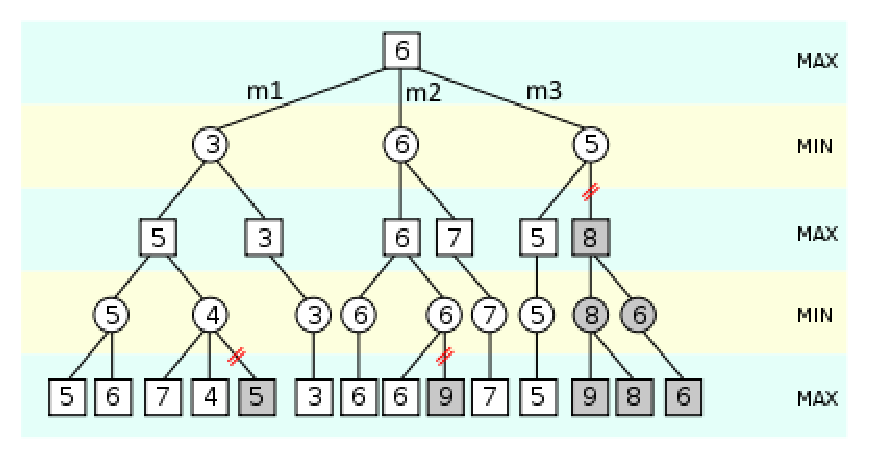
\includegraphics[scale=0.8]{contenido/cap3/imagenes/podaalfabeta.eps}
	\caption{Poda alfa-beta aplicada a un árbol de juegos.}
	\label{fig:alfabeta}
\end{figure}

En los agentes desarrollados esto no siempre es así y puede ocurrir que el mejor movimiento devuelto por minimax sea distinto del mejor movimiento devuelto por alfa-beta (pero ambos tendrán el mismo valor de evaluación); esto se debe a que los sucesores son generados en orden aleatorio y además, en el caso de que más de un estado tenga la misma evaluación, minimax cogerá el último sucesor que evalúe mientras que alfa-beta puede podar esa rama si encontró otro nodo con la misma evaluación.

La eficacia de la poda alfa-beta depende mucho del orden en el que se examinan los sucesores.
Una posible mejora del algoritmo sería examinar primero los sucesores que probablemente sean mejores.
Para una búsqueda en un árbol a profundidad \textit{p} y un factor de ramificación \textit{b}, en el mejor caso (los nodos están ordenados de mejor a peor), alfa-beta tiene que examinar $O(b^{p/2})$ nodos para escoger el mejor movimiento, en vez de $O(b^p)$ para minimax.% lo que reduce a la mitad el tiempo necesario.
En los algoritmos desarrollados donde los sucesores se examinan en orden aleatorio, el número total de nodos examinados es de $O(b^{3p/4})$.
Por último, en el peor de los casos, donde no se realiza ninguna poda, la complejidad es la misma que en minimax: $O(b^p)$.

\bigskip
A continuación se presentan los agentes que emplean la técnica de la poda alfa-beta, al igual que ocurría con minimax se trata de dos agentes con características diferentes: uno con un límite en la profundidad de búsqueda y otro con un tiempo limitado de búsqueda.

\subsubsection{Alfa-beta con profundidad máxima de búsqueda}
\label{sssec:profundidad_maxima_busqueda_alfabeta}
Este agente emplea el algoritmo negamax con poda alfa-beta incluida para realizar una búsqueda en el árbol de juegos a una profundidad máxima indicada a partir de la posición actual.

La lógica del agente es la misma que la explicada para el agente minimax con profundidad máxima de búsqueda (apartado~\ref{sssec:profundidad_maxima_busqueda}), con el incentivo de que incorpora la poda alfa-beta.

\subsubsection{Alfa-beta con límite de tiempo}
\label{sssec:limite_tiempo_alfabeta}
El segundo agente también emplea el algoritmo negamax con poda alfa-beta y dispone de un tiempo limitado para realizar la búsqueda del mejor movimiento en el árbol de juegos.

El agente tiene las mismas características que el agente minimax con límite de tiempo (descrito en el apartado~\ref{sssec:limite_tiempo}), pero incluyendo además las ventajas de la poda alfa-beta.
